%!TEX root=../../autopilot.tex

\section{Network Latency}
\label{sec:networklatency}


\begin{margintable}[2.5cm]
\caption{Network Test Materials}
\label{tab:netmaterials}
\noindent\begin{tabularx}{\linewidth}{lX}%
\toprule
\textbf{Router} & \href{https://www.tp-link.com/us/home-networking/wifi-router/archer-c7/}{TP-Link AC1750} \\
\href{https://wiki.auto-pi-lot.com/index.php/NTP}{\textbf{Chrony}} & 4.0 \\
\textbf{zmq} & 22.3.0 \\
\textbf{Code} & \href{https://github.com/auto-pi-lot/plugin-paper/blob/main/plugin_paper/tasks/network.py}{Network\_Latency} \\
\textbf{Replicate} & Assign task to subject from Terminal, start Task. \\
\bottomrule
\end{tabularx}
\end{margintable}

To support data-intensive tasks like those that require online processing of video or electrophysiological data, the networking modules at the core of Autopilot need high bandwidth and low latency. 

To test the latency of Autopilot's networking modules, we switch from "script mode" to "Task mode" (Table \ref{tab:netmaterials}). Tasks are useful for encapsulating multistage routines across multiple devices that would be hard to coordinate with scripts alone. Our \texttt{Network\_Latency} task consists of one "leader" pilot sending timestamped messages to a "follower" pilot which returns the timestamp marking when it received the message. The two pis communicate via two directly connected \texttt{Net\_Node}s (rather than routing each message through agent-level \texttt{Station} objects) after the leader pi initiates the follower with a multihop "START" message routed through a Terminal agent containing the task and networking parameters. We measured latency using software timestamps while synchronizing the clocks of the two pis with Chrony, an \href{https://en.wikipedia.org/wiki/Network\_Time\_Protocol}{NTP} daemon previously measured to synchronize Raspberry Pis within dozens of microseconds\citep{soaresAnalysisTimekeepingExperimentation2020}\sidenote{Our sync is likely to be near to or better than that reported in \citep{soaresAnalysisTimekeepingExperimentation2020}: in addition to a quiet network, we configured chrony to poll more frequently and tolerate a smaller error than default}, with the leader pi hosting an NTP server and the follower pi synchronizing its clock solely from the leader. We documented this \href{https://wiki.auto-pi-lot.com/index.php/NTP}{on the wiki} too, since synchronization is a universal problem in multi-computer experiments.

\begin{figure}
\caption{Network latency from when a message is sent from one pilot to when it is received by another. Messages took 0.975ms to send and receive (median, $\pm$ 0.1 IQR, n=10,000, overlaid numbers and red shading in density plot indicate quartiles). There is a clear bimodality in latencies for individual messages (black dots, jittered in y-axis) with unclear cause.}
\label{fig:netlag}
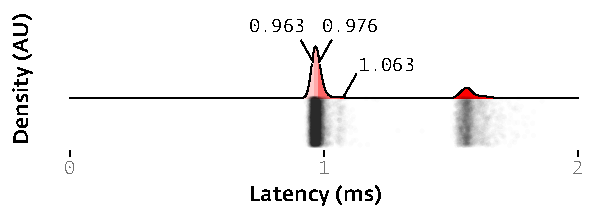
\includegraphics{figures/networking_latency_raster.pdf}
\end{figure}

Point to point latency was 0.975ms (median, $\pm$ 0.1 IQR, n=10,000, Figure \ref{fig:netlag}) with some clear bimodality where a subset of messages (\~2,300 of 10,000) took longer (median 1.567ms). The source of the bimodality is unclear to us, though it could be due to network congestion or interruption by other processes as the networking modules are not run in their own process like the sound server. This latency includes message serialization and deserialization by the builtin JSON library, which is on the order of roughly 100$\mu s$ each for even the very small messages sent in this test. In future versions we will explore other serialization tools like \href{https://msgpack.org/}{msgpack} and offer them as alternate serialization backends.